\documentclass[problem]{mcs}

%%%%%%%%%%%%%%%%%%%%%%%%%%%%%%%%%%%%%%%%%%%%%%%%%%%%%%%%%%%%%%%%%%%%%
% Problem starts here
%%%%%%%%%%%%%%%%%%%%%%%%%%%%%%%%%%%%%%%%%%%%%%%%%%%%%%%%%%%%%%%%%%%%%


\begin{problem}
\PTAGfilename{}
\PTAGhistory{}
%\PTAGkeywords{}
%
\begin{definition}
 The recursive data type, $\btg$, of \term{binary trees} with
 leaf labels, $L$ is defined recursively as follows:
\begin{itemize}

\item \textbf{Base case:}
$\ang{\texttt{leaf},l} \in \btg$, for all $l\in L$.

\item \textbf{Constructor case:} If $G_1,G_2 \in \btg$, then
\[
\ang{\texttt{bintree},G_1,G_2} \in \btg.
\]
\end{itemize}

The \term{size}, $\card{G}$, of $G \in \btg$ is defined recursively on
this definition by:

\begin{itemize}
\item \textbf{Base case:}
\[
\card{\ang{\texttt{leaf}, l}} \eqdef \eqdef l, \quad \text{ for all} l \in L.
\]

\item \textbf{Constructor case:}
\[
\card{\ang{\texttt{bintree}, G_1, G_2}} \eqdef \card{G_1}+ \card{G_2} + 1.
\]
\end{itemize}
\end{definition}

For example, for the size of the $\btg$, $G$, pictured in
Figure~\ref{CP0303:small-tree}, is 7.

\begin{figure}[htbp]
\centering 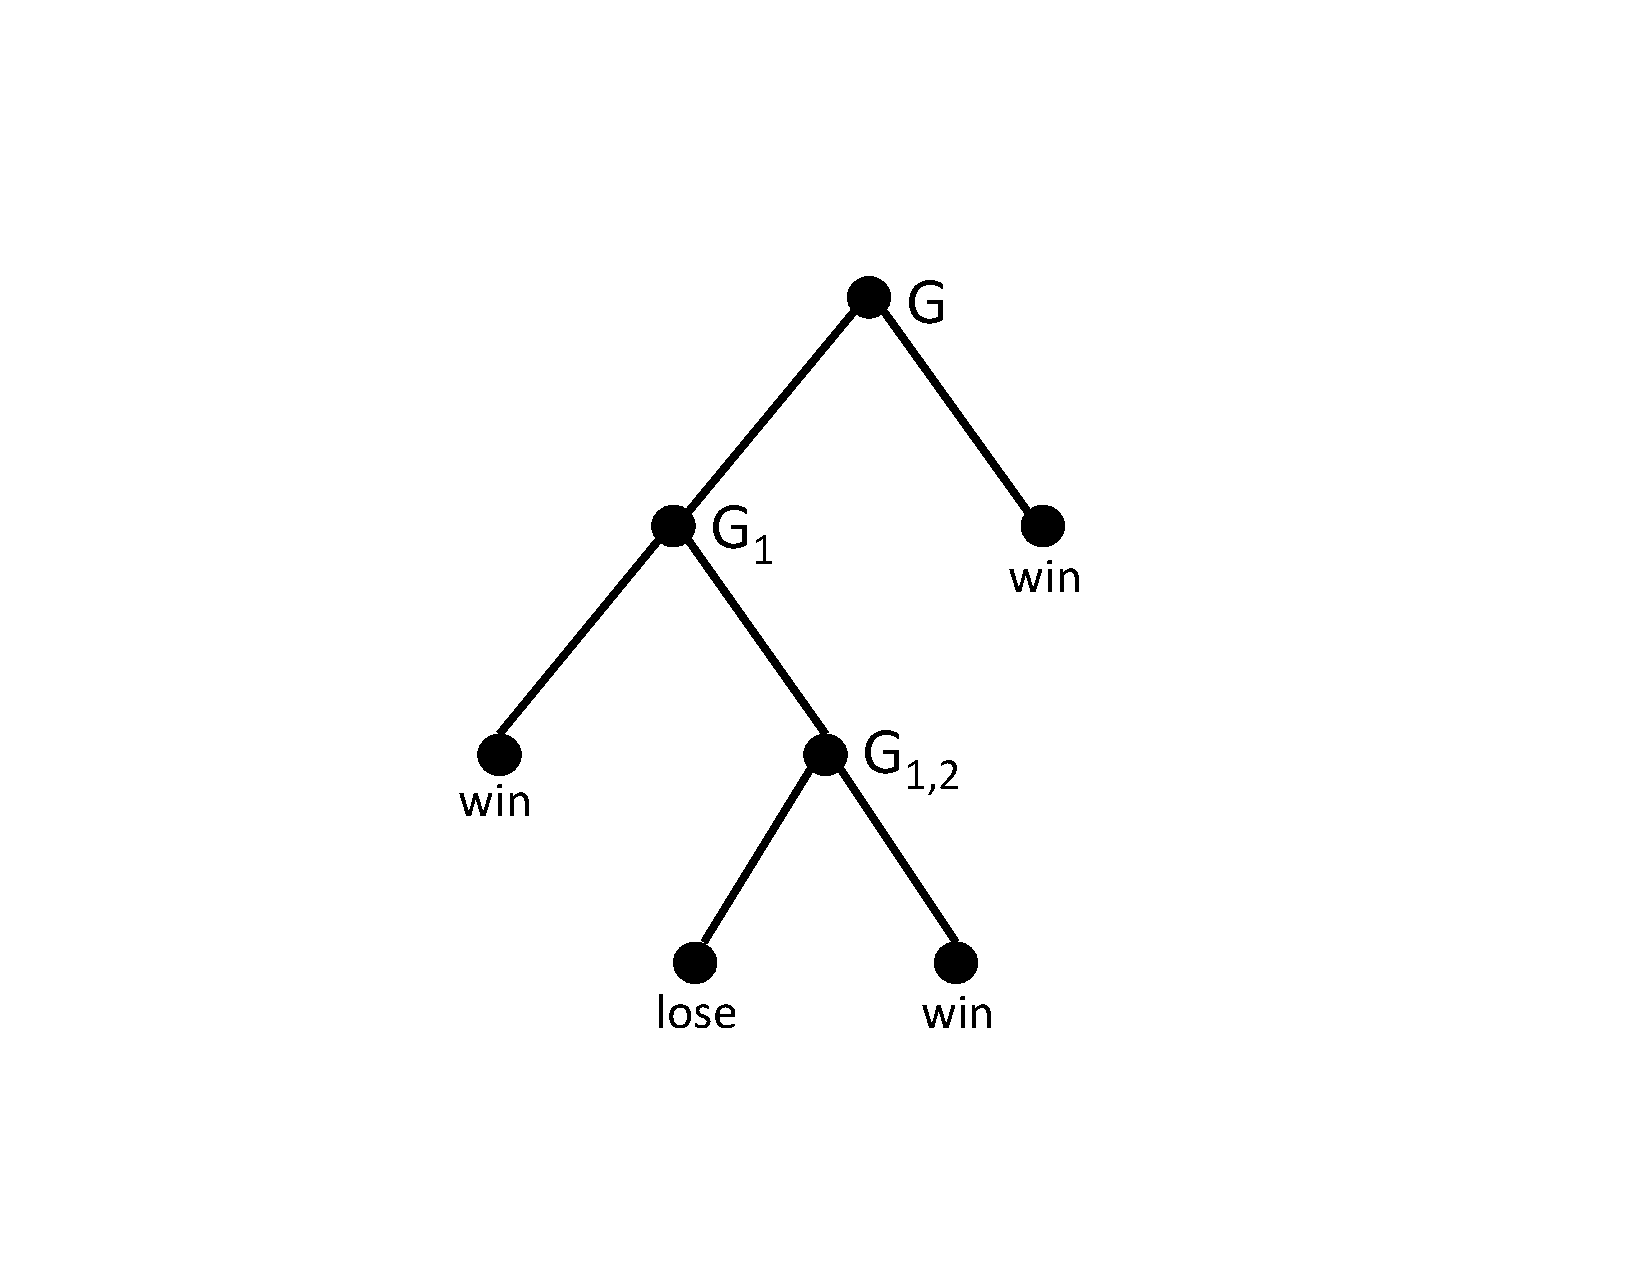
\includegraphics[height=3in]{figures/binary-game-tree.pdf}
\caption{\emph{A picture of a binary tree $w$.}}
\label{CP0303:small-tree}
\end{figure}

\bparts
\ppart Write out (using angle brackets and labels \texttt{bintree},
\texttt{leaf}, etc.) the $\btg$, $G$, pictured in Figure~\ref{CP0303:small-tree}.

\solution{
\begin{equation}
\begin{split}
\langle\texttt{bintree}, & \langle\texttt{bintree}, \ang{\texttt{leaf, win}},\\
  & \hspace{5em} \ang{\texttt{bintree}, \ang{\texttt{leaf, lose}}, \ang{\texattt{leaf,
       win}}}\rangle,\\
  & \ang{\texttt{leaf, win}}\rangle
\end{split}
\end{equation}
}

\eparts

The value of $\text{flatten}(G)$ for $G \in \btg$ is the sequence of
labels in $L$ of the leaves of $G$.  For example, for the $\btg$, $G$,
pictured in Figure~\ref{CP0303:small-tree},
\[
\text{flatten}(G) = (\texttt{win}, \texttt{lose}, \texttt{win}, \texttt{win}).
\]  %Need updating for general labels

\bparts

\ppart
Give a recursive definition of flatten.  (You may use the operation of
\emph{concatenation} (append) of two sequences.)

\solution{ Define flatten recursively on the definition of $\btg$.

\begin{itemize}

\item \textbf{Base case:}
\begin{align*}
a\text{flatten}(\ang{\texttt{leaf}, \texttt{win}}) & \eqdef (\texttt{win}),\\
\text{flatten}(\ang{\texttt{leaf}, \texttt{lose}})& \eqdef (\texttt{lose}).
\end{align*}

\item \textbf{Constructor case:}
\[
\text{flatten}(\ang{\texttt{bintree}, G_1, G_2}) \eqdef
\text{flatten}(G_1)\text{flatten}(G_2)
\] 
where $\text{flatten}(G_1)\text{flatten}(G_2)$ is the concatenation of the
the two sequences of leaf labels, that is the sequence of labels in
$\text{flatten}(G_1)$ followed by the labels in $\text{flatten}(G_2)$.
\end{itemize}
}

\ppart Prove by structural induction on the definitions of flatten and
size that
\begin{equation}\label{CP0303:2gg1}
2\cdot \text{length}(\text{flatten}(G)) = \card{G}+1.
\end{equation}

\solution{ The proof is by structural induction on the given function
  definitions.  The induction hypothesis is the equation~\eqref{CP0303:2gg1}.

\begin{itemize}
\item \textbf{Base cases:}
\[2 \cdot \text{length}(\text{flatten}(\ang{\texttt{leaf},
    \text{label}})) = 2\cdot \text{length}((\text{label})) = 2 \cdot 1 =
  2 = 1 + 1 = \card{\ang{\texttt{leaf}, \text{label}}} + 1.
\]
So~\eqref{CP0303:2gg1} holds in the base cases.

\item \textbf{Constructor case:}
Say $G = \ang{\texttt{bintree}, G_1, G_2}$ where we assume the Structural
Induction hypothesis that $G_1$ and $G_2$ satisfy~\eqref{CP0303:2gg1}.  Now,
\begin{align*}
\lefteqn{2\cdot \text{length}(\text{flatten}(G))}\\
  & = 2 \cdot \text{length}(\text{flatten}(\ang{\texttt{bintree}, G_1, G_2}))\\
  & = 2\cdot \text{length}(\text{flatten}(G_1)\text{flatten}(G_2))
        & \text{(def of flatten)}\\
  & = 2\cdot \text{length}(\text{flatten}(G_1))+
     2 \cdot \text{length}(\text{flatten}(G_2))
        & \text{(length of a string)}\\
  & = (\card{G_1}+1) + \card{G_2}+1 & \text{(Structural Induction hyp.)}\\
  & = (\card{G_1} + \card{G_2}+1) +1\\
  & = \card{\ang{\texttt{bintree}, G_1, G_2}} + 1
           & \text{(def. of $\card{\ang{\text{bintree},\dots}}$)}\\
  & = \card{G} +1,
\end{align*}
proving that~\eqref{CP0303:2gg1} holds for $G$.
This completes the proof for the Constructor cases.
\end{itemize}

We conclude by Structural Induction that equation~\eqref{CP0303:2gg1} holds for
all $G \in \btg$.}
\eparts
\end{problem}

%%%%%%%%%%%%%%%%%%%%%%%%%%%%%%%%%%%%%%%%%%%%%%%%%%%%%%%%%%%%%%%%%%%%%
% Problem ends here
%%%%%%%%%%%%%%%%%%%%%%%%%%%%%%%%%%%%%%%%%%%%%%%%%%%%%%%%%%%%%%%%%%%%%

\endinput
